\documentclass[preprint]{sigplanconf}

\usepackage[utf8]{inputenc}
% the following standard packages may be helpful, but are not required
\usepackage{longtable}
%\usepackage{mathtools}
%\usepackage{multicol}
%\usepackage{multirow}
\usepackage{booktabs}
%\usepackage{courier}
%\usepackage[scaled]{helvet}
%\usepackage{url}
\usepackage{listings}
%\usepackage{enumitem}
%\usepackage{mdwlist} % tighter description environment (starred)
%
\usepackage{graphicx}
\usepackage{softdev}
\usepackage{amsmath}
%\usepackage{mdwlist}
%\usepackage{pifont}
\usepackage{xspace}

\newcommand{\kalibera}{Kalibera \& Jones\xspace}
\newcommand{\krun}{Krun\xspace}
\newcommand{\hypone}{H1\xspace}
\newcommand{\hyptwo}{H2\xspace}
\newcommand{\binarytrees}{\emph{binary trees}\xspace}
\newcommand{\richards}{\emph{Richards}\xspace}
\newcommand{\spectralnorm}{\emph{spectralnorm}\xspace}
\newcommand{\nbody}{\emph{n-body}\xspace}
\newcommand{\fasta}{\emph{fasta}\xspace}
\newcommand{\fannkuch}{\emph{fannkuch redux}\xspace}
\newcommand{\bencherthree}{Linux1/i7-4709K\xspace}
\newcommand{\bencherfive}{Linux2/i7-4790\xspace}
\newcommand{\benchersix}{OpenBSD/i7-4790\xspace}
\newcommand{\bencherseven}{ARM\edd{XXX name properly if used}\xspace}

\lstset{
    basicstyle=\tt\scriptsize,
    xleftmargin=2em,
    framexleftmargin=1.5em,
    numberstyle=\scriptsize\tt\color{gray},
    captionpos=b,
    escapeinside={{<!}{!>}},
}

\SDShowCommentTags{default}  %final

\begin{document}

\title{Virtual Machine Warmup Blows Hot and Cold}

\authorinfo{Edd Barrett}
{Software Development Team, Department of Informatics, King's College London}{\texttt{http://eddbarrett.co.uk/}}

\authorinfo{Carl Friedrich Bolz}
{Software Development Team, Department of Informatics, King's College London}{\texttt{http://cfbolz.de/}}

\authorinfo{Rebecca Killick}
{Department of Mathematics and Statistics, University of Lancaster}{\texttt{http://www.lancs.ac.uk/\~{}killick/}}

\authorinfo{Vincent Knight}
{School of Mathematics, Cardiff University}{\texttt{http://vknight.org/}}

\authorinfo{Sarah Mount}
{Software Development Team, Department of Informatics, King's College London}{\texttt{http://snim2.org/}}

\authorinfo{Laurence Tratt}
{Software Development Team, Department of Informatics, King's College London}{\texttt{http://tratt.net/laurie/}}


\maketitle

\section{Introduction}
\label{sec:intro}

Many modern languages are implemented as Virtual Machines (VMs) which use a
Just-In-Time (JIT) compiler to translate `hot' parts of a program into efficient
machine code at run-time. Since it takes time to determine which parts of the
program are hot, and then compile them, programs which are JIT compiled are
said to be subject to a \emph{warmup} phase. The traditional view of
JIT compiled VMs is that program execution is slow during the warmup phase, and
fast afterwards, when \emph{peak performance} is said to have been reached
(see Figure~\ref{fig:trad} for a simplified view of this).
This traditional view underlies most benchmarking of JIT compiled VMs, which
generally aim to measure peak performance.
Benchmarking methodologies usually
require running benchmarks several times within a single VM process, and
discarding any timing data collected before warmup is complete.

The fundamental aim of this paper is to test the following hypothesis, which captures a constrained
notion of the traditional notion of warmup:
\begin{description}
  \item[\hypone] Small, deterministic programs exhibit traditional warmup behaviour.
\end{description}
In order to test this hypothesis, we present a carefully designed
experiment where a number of simple benchmarks are run on a variety of
VMs for a large number of \emph{in-process iterations} and repeated using fresh
\emph{process executions} (i.e.~each process execution runs multiple in-process
iterations). Note that we deliberately treat VMs as black
boxes: we simply run benchmarks and record timing data. It is not our intention
to understand the effects we see in the resulting timing data, for the simple
reason that we are not experts in most of the VMs under investigation. Even were
we experts, understanding some of the resulting data could take many person
months of effort per VM.
%From this we obtain \emph{time series} data, to which we apply a
%number of statistical techniques that have not previously been applied
%in the context of VM benchmarking.

\begin{figure}[t]
\centering
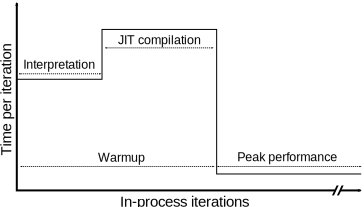
\includegraphics[width=.5\textwidth]{img/picturebook_warmup}
\caption{The traditional notion of warmup: a program starts slowly executing in
an interpreter; once hot parts of the program are identified, they are
translated by the JIT compiler to machine code; at this point warmup
is said to have completed, and peak performance reached.}
\label{fig:trad}
\end{figure}

We expected our experiment to validate Hypothesis H1, allowing us to
easily compare warmup across VMs. While some benchmarks on some VMs run as per
traditional expectations, we found a number of surprising cases. At
the most extreme, some benchmarks never warm up, staying at their initial performance
levels indefinitely and some even slowdown. Of the eight
VMs we looked at, none consistently warmed under the traditional model.

Our results clearly show that the traditional view of warmup is no longer valid (and, perhaps,
that it may not have held in the past). We are not aware that anyone has systematically noted this
problem before, let alone take it into account when benchmarking. This suggests
that many published VM benchmarks (including our own) may have presented
results which are misleading in some situations.

A reasonable question, therefore, is whether inaccuracies in VM benchmarking are of anything
other than academic interest. We believe that accurate VM benchmarking is needed
by both VM authors and many end users. When
implementing optimisations, VM authors need to know if their optimisations have
had the intended effect or not: since many optimisations, in isolation, have only a
small effect, accurate benchmarking is vital. Our results suggest that decisions
about the effectiveness of an optimisation may sometimes be made based on
unreliable data.
It is likely that this has caused some ineffective, and perhaps even some deleterious,
optimisations to be included in VMs. Many end users have workloads that are more
sensitive to latency than throughput. For example, users running games (or other
soft real-time systems) require predictable performance. Our results show that some
VMs JIT compile programs that have unpredictable long-term performance.

% XXX needs at-least one
\cite{test123}

\bibliographystyle{plain}
\bibliography{bib}

\end{document}

